% Created by tikzDevice version 0.6.2-92-0ad2792 on 2012-09-16 01:19:14
% !TEX encoding = UTF-8 Unicode
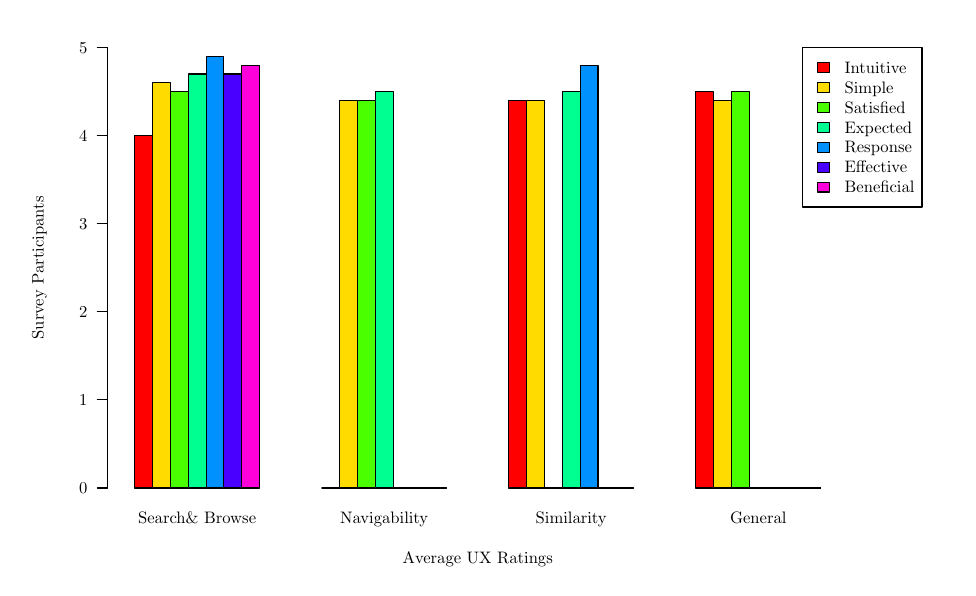
\begin{tikzpicture}[x=1pt,y=1pt]
\definecolor[named]{fillColor}{rgb}{1.00,1.00,1.00}
\path[use as bounding box,fill=fillColor,fill opacity=0.00] (0,0) rectangle (332.44,195.13);
\begin{scope}
\path[clip] (  0.00,  0.00) rectangle (332.44,195.13);
\definecolor[named]{drawColor}{rgb}{0.00,0.00,0.00}
\definecolor[named]{fillColor}{rgb}{1.00,0.00,0.00}

\path[draw=drawColor,line width= 0.4pt,line join=round,line cap=round,fill=fillColor] ( 38.71, 28.80) rectangle ( 45.15,156.10);
\definecolor[named]{fillColor}{rgb}{1.00,0.86,0.00}

\path[draw=drawColor,line width= 0.4pt,line join=round,line cap=round,fill=fillColor] ( 45.15, 28.80) rectangle ( 51.59,175.20);
\definecolor[named]{fillColor}{rgb}{0.29,1.00,0.00}

\path[draw=drawColor,line width= 0.4pt,line join=round,line cap=round,fill=fillColor] ( 51.59, 28.80) rectangle ( 58.02,172.02);
\definecolor[named]{fillColor}{rgb}{0.00,1.00,0.57}

\path[draw=drawColor,line width= 0.4pt,line join=round,line cap=round,fill=fillColor] ( 58.02, 28.80) rectangle ( 64.46,178.38);
\definecolor[named]{fillColor}{rgb}{0.00,0.57,1.00}

\path[draw=drawColor,line width= 0.4pt,line join=round,line cap=round,fill=fillColor] ( 64.46, 28.80) rectangle ( 70.90,184.75);
\definecolor[named]{fillColor}{rgb}{0.29,0.00,1.00}

\path[draw=drawColor,line width= 0.4pt,line join=round,line cap=round,fill=fillColor] ( 70.90, 28.80) rectangle ( 77.33,178.38);
\definecolor[named]{fillColor}{rgb}{1.00,0.00,0.86}

\path[draw=drawColor,line width= 0.4pt,line join=round,line cap=round,fill=fillColor] ( 77.33, 28.80) rectangle ( 83.77,181.56);
\definecolor[named]{fillColor}{rgb}{1.00,0.00,0.00}

\path[draw=drawColor,line width= 0.4pt,line join=round,line cap=round,fill=fillColor] (106.30, 28.80) rectangle (112.74, 28.80);
\definecolor[named]{fillColor}{rgb}{1.00,0.86,0.00}

\path[draw=drawColor,line width= 0.4pt,line join=round,line cap=round,fill=fillColor] (112.74, 28.80) rectangle (119.17,168.83);
\definecolor[named]{fillColor}{rgb}{0.29,1.00,0.00}

\path[draw=drawColor,line width= 0.4pt,line join=round,line cap=round,fill=fillColor] (119.17, 28.80) rectangle (125.61,168.83);
\definecolor[named]{fillColor}{rgb}{0.00,1.00,0.57}

\path[draw=drawColor,line width= 0.4pt,line join=round,line cap=round,fill=fillColor] (125.61, 28.80) rectangle (132.05,172.02);
\definecolor[named]{fillColor}{rgb}{0.00,0.57,1.00}

\path[draw=drawColor,line width= 0.4pt,line join=round,line cap=round,fill=fillColor] (132.05, 28.80) rectangle (138.48, 28.80);
\definecolor[named]{fillColor}{rgb}{0.29,0.00,1.00}

\path[draw=drawColor,line width= 0.4pt,line join=round,line cap=round,fill=fillColor] (138.48, 28.80) rectangle (144.92, 28.80);
\definecolor[named]{fillColor}{rgb}{1.00,0.00,0.86}

\path[draw=drawColor,line width= 0.4pt,line join=round,line cap=round,fill=fillColor] (144.92, 28.80) rectangle (151.36, 28.80);
\definecolor[named]{fillColor}{rgb}{1.00,0.00,0.00}

\path[draw=drawColor,line width= 0.4pt,line join=round,line cap=round,fill=fillColor] (173.89, 28.80) rectangle (180.32,168.83);
\definecolor[named]{fillColor}{rgb}{1.00,0.86,0.00}

\path[draw=drawColor,line width= 0.4pt,line join=round,line cap=round,fill=fillColor] (180.32, 28.80) rectangle (186.76,168.83);
\definecolor[named]{fillColor}{rgb}{0.29,1.00,0.00}

\path[draw=drawColor,line width= 0.4pt,line join=round,line cap=round,fill=fillColor] (186.76, 28.80) rectangle (193.20, 28.80);
\definecolor[named]{fillColor}{rgb}{0.00,1.00,0.57}

\path[draw=drawColor,line width= 0.4pt,line join=round,line cap=round,fill=fillColor] (193.20, 28.80) rectangle (199.63,172.02);
\definecolor[named]{fillColor}{rgb}{0.00,0.57,1.00}

\path[draw=drawColor,line width= 0.4pt,line join=round,line cap=round,fill=fillColor] (199.63, 28.80) rectangle (206.07,181.56);
\definecolor[named]{fillColor}{rgb}{0.29,0.00,1.00}

\path[draw=drawColor,line width= 0.4pt,line join=round,line cap=round,fill=fillColor] (206.07, 28.80) rectangle (212.51, 28.80);
\definecolor[named]{fillColor}{rgb}{1.00,0.00,0.86}

\path[draw=drawColor,line width= 0.4pt,line join=round,line cap=round,fill=fillColor] (212.51, 28.80) rectangle (218.94, 28.80);
\definecolor[named]{fillColor}{rgb}{1.00,0.00,0.00}

\path[draw=drawColor,line width= 0.4pt,line join=round,line cap=round,fill=fillColor] (241.47, 28.80) rectangle (247.91,172.02);
\definecolor[named]{fillColor}{rgb}{1.00,0.86,0.00}

\path[draw=drawColor,line width= 0.4pt,line join=round,line cap=round,fill=fillColor] (247.91, 28.80) rectangle (254.35,168.83);
\definecolor[named]{fillColor}{rgb}{0.29,1.00,0.00}

\path[draw=drawColor,line width= 0.4pt,line join=round,line cap=round,fill=fillColor] (254.35, 28.80) rectangle (260.78,172.02);
\definecolor[named]{fillColor}{rgb}{0.00,1.00,0.57}

\path[draw=drawColor,line width= 0.4pt,line join=round,line cap=round,fill=fillColor] (260.78, 28.80) rectangle (267.22, 28.80);
\definecolor[named]{fillColor}{rgb}{0.00,0.57,1.00}

\path[draw=drawColor,line width= 0.4pt,line join=round,line cap=round,fill=fillColor] (267.22, 28.80) rectangle (273.66, 28.80);
\definecolor[named]{fillColor}{rgb}{0.29,0.00,1.00}

\path[draw=drawColor,line width= 0.4pt,line join=round,line cap=round,fill=fillColor] (273.66, 28.80) rectangle (280.09, 28.80);
\definecolor[named]{fillColor}{rgb}{1.00,0.00,0.86}

\path[draw=drawColor,line width= 0.4pt,line join=round,line cap=round,fill=fillColor] (280.09, 28.80) rectangle (286.53, 28.80);
\end{scope}
\begin{scope}
\path[clip] (  0.00,  0.00) rectangle (332.44,195.13);
\definecolor[named]{drawColor}{rgb}{0.00,0.00,0.00}

\node[text=drawColor,anchor=base,inner sep=0pt, outer sep=0pt, scale=  0.60] at ( 61.24, 15.84) {Search\& Browse};

\node[text=drawColor,anchor=base,inner sep=0pt, outer sep=0pt, scale=  0.60] at (128.83, 15.84) {Navigability};

\node[text=drawColor,anchor=base,inner sep=0pt, outer sep=0pt, scale=  0.60] at (196.41, 15.84) {Similarity};

\node[text=drawColor,anchor=base,inner sep=0pt, outer sep=0pt, scale=  0.60] at (264.00, 15.84) {General};
\end{scope}
\begin{scope}
\path[clip] (  0.00,  0.00) rectangle (332.44,195.13);
\definecolor[named]{drawColor}{rgb}{0.00,0.00,0.00}

\node[text=drawColor,anchor=base,inner sep=0pt, outer sep=0pt, scale=  0.60] at (162.62,  1.44) {Average UX Ratings};

\node[text=drawColor,rotate= 90.00,anchor=base,inner sep=0pt, outer sep=0pt, scale=  0.60] at (  5.76,108.36) {Survey Participants};
\end{scope}
\begin{scope}
\path[clip] (  0.00,  0.00) rectangle (332.44,195.13);
\definecolor[named]{drawColor}{rgb}{0.00,0.00,0.00}

\path[draw=drawColor,line width= 0.4pt,line join=round,line cap=round] ( 28.80, 28.80) -- ( 28.80,187.93);

\path[draw=drawColor,line width= 0.4pt,line join=round,line cap=round] ( 28.80, 28.80) -- ( 25.20, 28.80);

\path[draw=drawColor,line width= 0.4pt,line join=round,line cap=round] ( 28.80, 60.63) -- ( 25.20, 60.63);

\path[draw=drawColor,line width= 0.4pt,line join=round,line cap=round] ( 28.80, 92.45) -- ( 25.20, 92.45);

\path[draw=drawColor,line width= 0.4pt,line join=round,line cap=round] ( 28.80,124.28) -- ( 25.20,124.28);

\path[draw=drawColor,line width= 0.4pt,line join=round,line cap=round] ( 28.80,156.10) -- ( 25.20,156.10);

\path[draw=drawColor,line width= 0.4pt,line join=round,line cap=round] ( 28.80,187.93) -- ( 25.20,187.93);

\node[text=drawColor,anchor=base east,inner sep=0pt, outer sep=0pt, scale=  0.60] at ( 21.60, 26.73) {0};

\node[text=drawColor,anchor=base east,inner sep=0pt, outer sep=0pt, scale=  0.60] at ( 21.60, 58.56) {1};

\node[text=drawColor,anchor=base east,inner sep=0pt, outer sep=0pt, scale=  0.60] at ( 21.60, 90.39) {2};

\node[text=drawColor,anchor=base east,inner sep=0pt, outer sep=0pt, scale=  0.60] at ( 21.60,122.21) {3};

\node[text=drawColor,anchor=base east,inner sep=0pt, outer sep=0pt, scale=  0.60] at ( 21.60,154.04) {4};

\node[text=drawColor,anchor=base east,inner sep=0pt, outer sep=0pt, scale=  0.60] at ( 21.60,185.86) {5};
\end{scope}
\begin{scope}
\path[clip] (  0.00,  0.00) rectangle (332.44,195.13);
\definecolor[named]{drawColor}{rgb}{0.00,0.00,0.00}

\path[draw=drawColor,line width= 0.4pt,line join=round,line cap=round] (280.09,187.93) rectangle (323.16,130.33);
\definecolor[named]{fillColor}{rgb}{1.00,0.00,0.00}

\path[draw=drawColor,line width= 0.4pt,line join=round,line cap=round,fill=fillColor] (285.49,182.53) rectangle (289.81,178.93);
\definecolor[named]{fillColor}{rgb}{1.00,0.86,0.00}

\path[draw=drawColor,line width= 0.4pt,line join=round,line cap=round,fill=fillColor] (285.49,175.33) rectangle (289.81,171.73);
\definecolor[named]{fillColor}{rgb}{0.29,1.00,0.00}

\path[draw=drawColor,line width= 0.4pt,line join=round,line cap=round,fill=fillColor] (285.49,168.13) rectangle (289.81,164.53);
\definecolor[named]{fillColor}{rgb}{0.00,1.00,0.57}

\path[draw=drawColor,line width= 0.4pt,line join=round,line cap=round,fill=fillColor] (285.49,160.93) rectangle (289.81,157.33);
\definecolor[named]{fillColor}{rgb}{0.00,0.57,1.00}

\path[draw=drawColor,line width= 0.4pt,line join=round,line cap=round,fill=fillColor] (285.49,153.73) rectangle (289.81,150.13);
\definecolor[named]{fillColor}{rgb}{0.29,0.00,1.00}

\path[draw=drawColor,line width= 0.4pt,line join=round,line cap=round,fill=fillColor] (285.49,146.53) rectangle (289.81,142.93);
\definecolor[named]{fillColor}{rgb}{1.00,0.00,0.86}

\path[draw=drawColor,line width= 0.4pt,line join=round,line cap=round,fill=fillColor] (285.49,139.33) rectangle (289.81,135.73);

\node[text=drawColor,anchor=base west,inner sep=0pt, outer sep=0pt, scale=  0.60] at (295.21,178.66) {Intuitive};

\node[text=drawColor,anchor=base west,inner sep=0pt, outer sep=0pt, scale=  0.60] at (295.21,171.46) {Simple};

\node[text=drawColor,anchor=base west,inner sep=0pt, outer sep=0pt, scale=  0.60] at (295.21,164.26) {Satisfied};

\node[text=drawColor,anchor=base west,inner sep=0pt, outer sep=0pt, scale=  0.60] at (295.21,157.06) {Expected};

\node[text=drawColor,anchor=base west,inner sep=0pt, outer sep=0pt, scale=  0.60] at (295.21,149.86) {Response};

\node[text=drawColor,anchor=base west,inner sep=0pt, outer sep=0pt, scale=  0.60] at (295.21,142.66) {Effective};

\node[text=drawColor,anchor=base west,inner sep=0pt, outer sep=0pt, scale=  0.60] at (295.21,135.46) {Beneficial};
\end{scope}
\end{tikzpicture}
